 \documentclass{article}
\usepackage[utf8]{inputenc}
\usepackage[a4paper, total={7in, 10in}]{geometry}
\usepackage{braket}
\usepackage{xcolor}
\usepackage{amsmath}
\usepackage{amssymb}
\usepackage{amsfonts}
\usepackage{graphicx}
\usepackage{svg}
\usepackage{float}
\usepackage{tikz}
\usepackage[ruled,vlined]{algorithm2e}
\usepackage{multicol}
\usepackage[backend=biber,style=alphabetic,sorting=ynt]{biblatex}
\usepackage{xcolor}
%\addbibresource{sample.bib} %Import the bibliography file

\newcommand{\commentt}[1]{\textcolor{blue}{ \textbf{[COMMENT]} #1}}
\newcommand{\ctt}[1]{\commentt{#1}}
\newcommand{\prb}[1]{ \mathbf{Pr} \left[ {#1} \right]}
\newcommand{\onotation}[1]{\(\mathcal{O} \left( {#1}  \right) \)}
\newcommand{\ona}[1]{\onotation{#1}}
\newcommand{\PSI}{{\ket{\psi}}}
\newcommand{\LESn}{\ket{\psi_n}}
\newcommand{\LESa}{\ket{\phi_n}}
\newcommand{\LESs}{\frac{1}{\sqrt{n}}\sum_{i}{\ket{\left(0^{i}10^{n-i}\right)^{n}}}}
\newcommand{\Hn}{\mathcal{H}_{n}}
\newcommand{\Ep}{\frac{1}{\sqrt{2^n}}\sum^{2^n}_{x}{ \ket{xx}}}
\newcommand{\HON}{\ket{\psi_{\text{honest}}}}
\newcommand{\Lemma}{\paragraph{Lemma.}}


\setlength{\columnsep}{0.6cm}

\newcommand{\Gz}{ G_{z}^{\delta} } 

\begin{document}

\title{Quantum LTC With Positive Rate}
\author{David Ponarovsky}
\maketitle
%\begin{multicols*}{2}
\newcommand{ \Hw }{ \delta\Delta -\Delta^{\frac{1}{2}-\varepsilon}/\delta  }
	\newcommand{ \Nw }{ \Delta^{\frac{3}{2}-\varepsilon}} 
	  \newcommand{ \Gu } { \Gamma^{\cup} }
	  \newcommand{ \Guq } { \Gamma^{\cup, \square} }

    	\newcommand{ \Gsa } {\Gamma_{\square_{1}} }
	\newcommand{ \Gsb } {\Gamma_{\square_{2}} }
        \newcommand{ \Aa } { C_{A_{1}}}  
	\newcommand{ \Ab } { C_{A_{2}}}
	\newcommand{ \Ac } { C_{A_{3}}}
	\newcommand{ \Aab } { \Aa \otimes \Ab } 
	\newcommand{ \Aac } { \Aa \otimes \Ac }
	\newcommand{ \Aabc } { \Aa \otimes \Ab \otimes \Ac }
	\newcommand{ \Aabp } { \Aa^{\perp} \otimes \Ab^{\perp} } 
	\newcommand{ \Aacp } { \Aa^{\perp} \otimes \Ac^{\perp} }
	\newcommand{ \Aabcp } { \Aa^{\perp} \otimes \Ab^{\perp} \otimes \Ac^{\perp} }
	\newcommand{ \Aabpp } { \left( \Aabp \right)^\perp } 
	\newcommand{ \Aacpp } { \left( \Aacp \right)^\perp }
	\newcommand{ \Aabcpp } { \left( \Aabcp \right)^\perp }
	\newcommand{ \YY } {  y_{1}y_{2}^{\top} }
	\newcommand{ \ZZ } {  z_{1}z_{2}^{\top} } 
	\newcommand{ \TT } { \tilde{\tau} } 


  \paragraph{preamble.} preamble.  
  \begin{figure}[H]
            %\label{fig:square}
            \begin{center}
            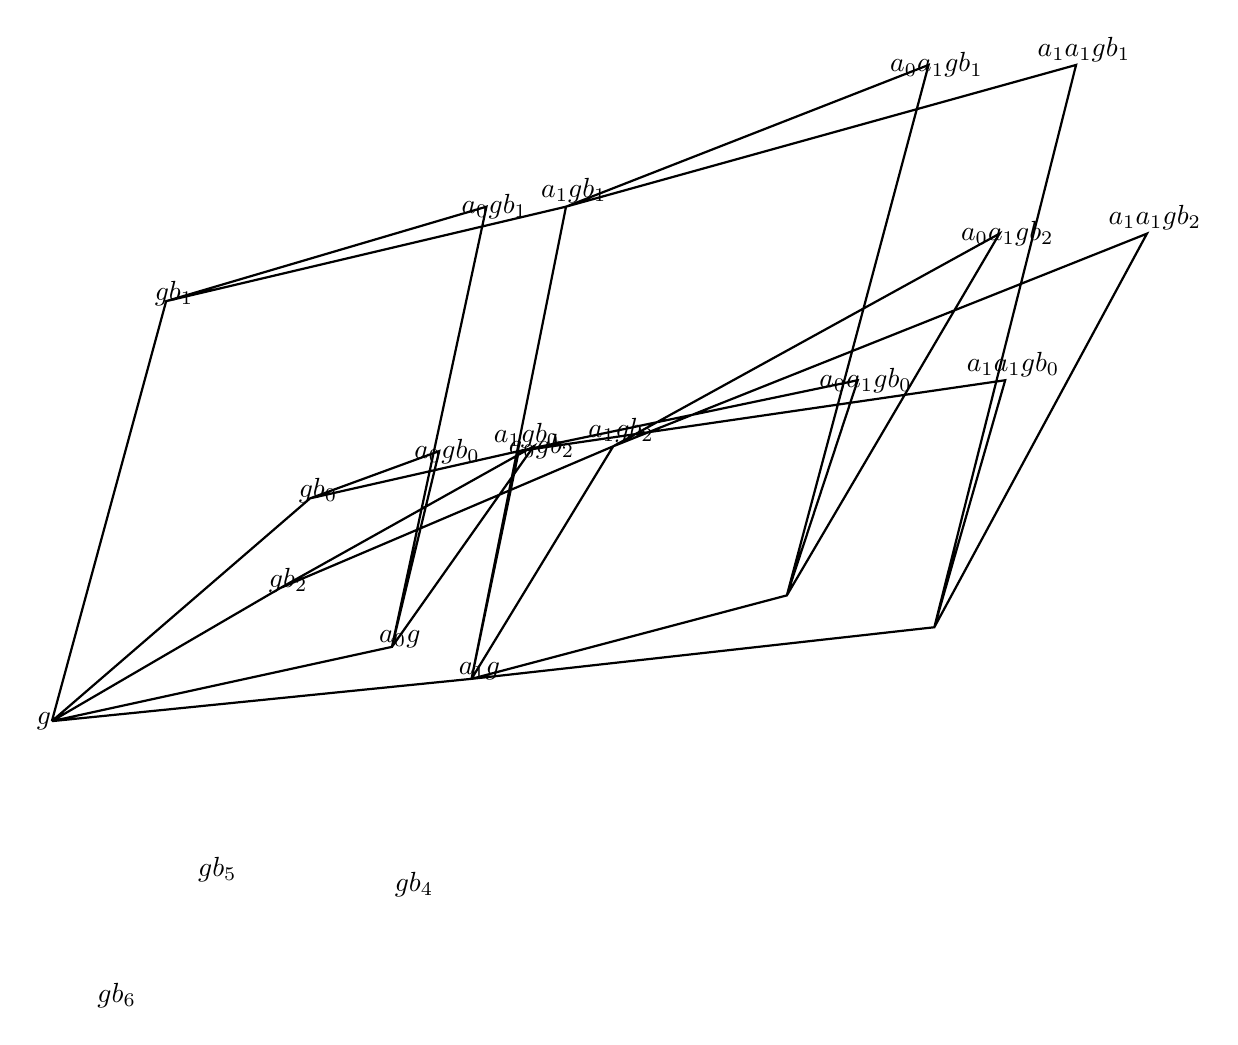
\begin{tikzpicture}
            \draw[thick](0,0)(0, 0) -- (3.2797999730966487,2.8295317336245875) -- (4.919062564693471,3.4295317336245876) -- (4.319062564693471,0.9434412119072285) -- (0, 0)
(0, 0) -- (1.4514484281033835,5.333740843151124) -- (5.5190625646934715,6.533740843151124) -- (4.319062564693471,0.9434412119072285) -- (0, 0)
(0, 0) -- (2.9018382469079365,1.6910390667884876) -- (6.119062564693471,3.4910390667884874) -- (4.319062564693471,0.9434412119072285) -- (0, 0)
(0, 0) -- (3.2797999730966487,2.8295317336245875) -- (5.929685547408452,3.4295317336245876) -- (5.329685547408452,0.537174906993143) -- (0, 0)
(0, 0) -- (1.4514484281033835,5.333740843151124) -- (6.5296855474084525,6.533740843151124) -- (5.329685547408452,0.537174906993143) -- (0, 0)
(0, 0) -- (2.9018382469079365,1.6910390667884876) -- (7.129685547408452,3.4910390667884874) -- (5.329685547408452,0.537174906993143) -- (0, 0)
(5.329685547408452, 0.537174906993143) -- (5.929685547408452,3.4295317336245876) -- (10.23433817528351,4.329531733624588) -- (9.33433817528351,1.5972134183799764) -- (5.329685547408452, 0.537174906993143)
(5.329685547408452, 0.537174906993143) -- (6.5296855474084525,6.533740843151124) -- (11.13433817528351,8.333740843151125) -- (9.33433817528351,1.5972134183799764) -- (5.329685547408452, 0.537174906993143)
(5.329685547408452, 0.537174906993143) -- (7.129685547408452,3.4910390667884874) -- (12.034338175283509,6.191039066788488) -- (9.33433817528351,1.5972134183799764) -- (5.329685547408452, 0.537174906993143)
(5.329685547408452, 0.537174906993143) -- (5.929685547408452,3.4295317336245876) -- (12.10719787842939,4.329531733624588) -- (11.20719787842939,1.1924742560275807) -- (5.329685547408452, 0.537174906993143)
(5.329685547408452, 0.537174906993143) -- (6.5296855474084525,6.533740843151124) -- (13.007197878429391,8.333740843151125) -- (11.20719787842939,1.1924742560275807) -- (5.329685547408452, 0.537174906993143)
(5.329685547408452, 0.537174906993143) -- (7.129685547408452,3.4910390667884874) -- (13.90719787842939,6.191039066788488) -- (11.20719787842939,1.1924742560275807) -- (5.329685547408452, 0.537174906993143)
;
\node at (5.019062564693471,3.4295317336245876) {$ a_{ 0  } gb_{ 0 } $};
\node at (5.619062564693471,6.533740843151124) {$ a_{ 0  } gb_{ 1 } $};
\node at (6.219062564693471,3.4910390667884874) {$ a_{ 0  } gb_{ 2 } $};
\node at (6.029685547408452,3.629531733624588) {$ a_{ 1  } gb_{ 0 } $};
\node at (6.629685547408452,6.733740843151124) {$ a_{ 1  } gb_{ 1 } $};
\node at (7.229685547408452,3.6910390667884876) {$ a_{ 1  } gb_{ 2 } $};
\node at (10.33433817528351,4.329531733624588) {$ a_{ 0  } a_{ 1 }gb_{ 0 } $};
\node at (11.23433817528351,8.333740843151125) {$ a_{ 0  } a_{ 1 }gb_{ 1 } $};
\node at (12.134338175283508,6.191039066788488) {$ a_{ 0  } a_{ 1 }gb_{ 2 } $};
\node at (12.20719787842939,4.529531733624588) {$ a_{ 1  } a_{ 1 }gb_{ 0 } $};
\node at (13.10719787842939,8.533740843151124) {$ a_{ 1  } a_{ 1 }gb_{ 1 } $};
\node at (14.00719787842939,6.391039066788488) {$ a_{ 1  } a_{ 1 }gb_{ 2 } $};
\node at (-0.1,0) {$ g $};
\node at (4.419062564693471,1.0434412119072285) {$ a_{ 0 }g $};
\node at (5.429685547408452,0.6371749069931429) {$ a_{ 1 }g $};
\node at (3.379799973096649,2.9295317336245876) {$ gb_{ 0 } $};
\node at (1.5514484281033836,5.433740843151123) {$ gb_{ 1 } $};
\node at (3.0018382469079365,1.7910390667884877) {$ gb_{ 2 } $};
\node at (4.599350222209558,-2.077437140657477) {$ gb_{ 4 } $};
\node at (2.101658733675802,-1.881727084098477) {$ gb_{ 5 } $};
\node at (0.8233934380414947,-3.4841033286795566) {$ gb_{ 6 } $};

            \end{tikzpicture}
            \end{center}
            \caption{Square of the complex, with edges $(g,ag), (agb, gb) \in E_A,
            (g,gb), (agb, ag) \in E_B.$ \label{fig:square}
            }
            \end{figure}
 \begin{figure}[H]
            %\label{fig:square}
            \begin{center}
            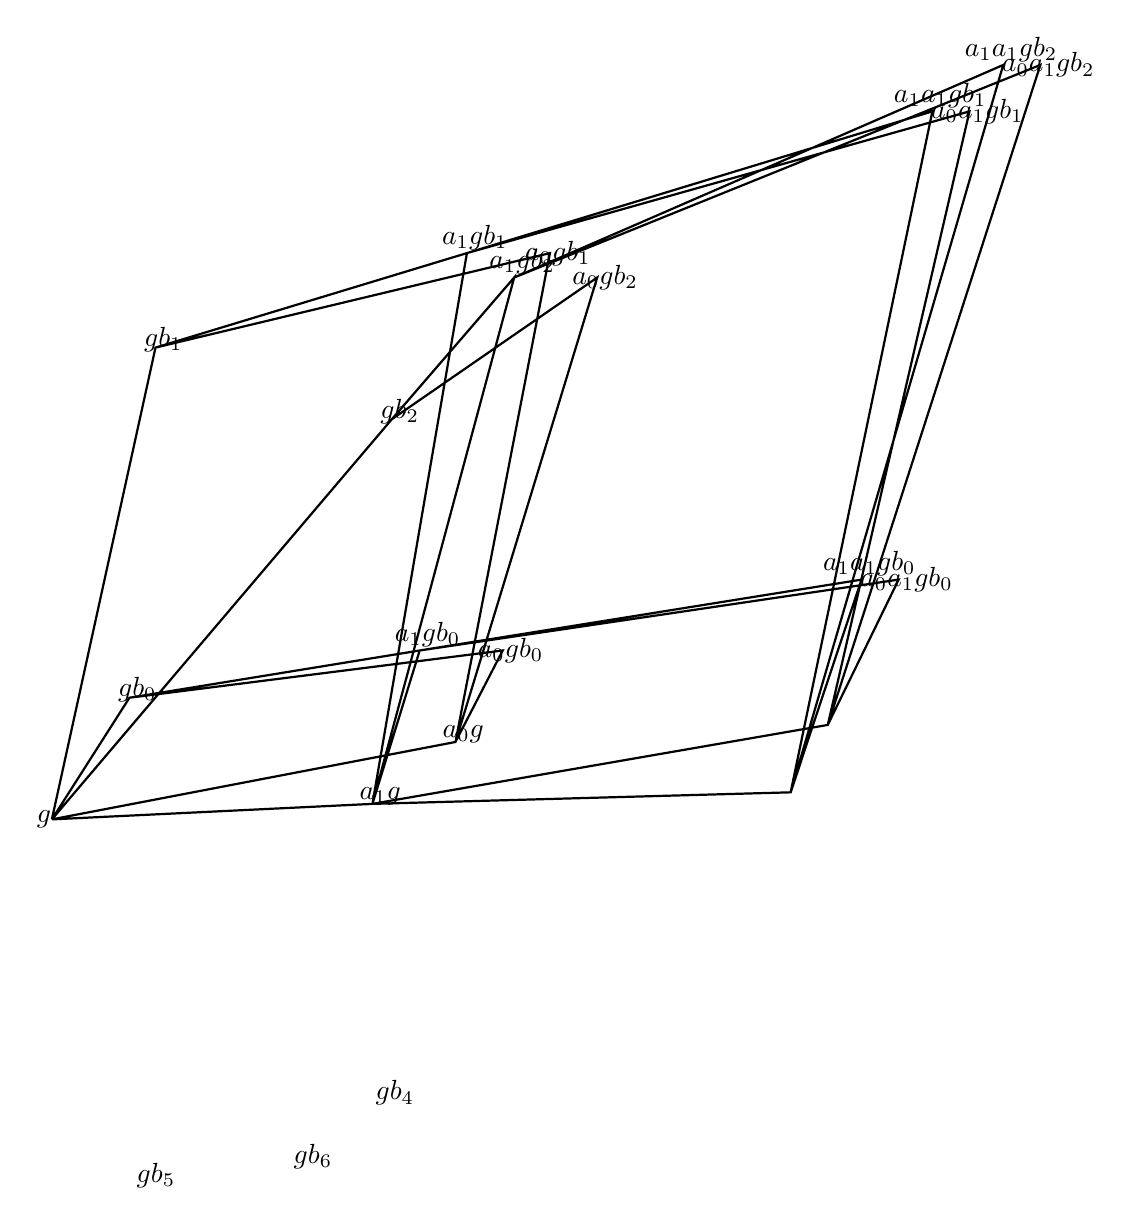
\begin{tikzpicture}
            \draw[thick](0,0)(0, 0) -- (0.9854202414966068,1.5449049914338562) -- (5.725514485599078,2.1449049914338563) -- (5.125514485599078,0.9827602592873228) -- (0, 0)
(0, 0) -- (1.31616594136513,5.991650724903537) -- (6.325514485599078,7.191650724903537) -- (5.125514485599078,0.9827602592873228) -- (0, 0)
(0, 0) -- (4.317235649008296,5.081312591835687) -- (6.925514485599078,6.8813125918356866) -- (5.125514485599078,0.9827602592873228) -- (0, 0)
(0, 0) -- (0.9854202414966068,1.5449049914338562) -- (4.671172602146307,2.1449049914338563) -- (4.071172602146308,0.1968232832143524) -- (0, 0)
(0, 0) -- (1.31616594136513,5.991650724903537) -- (5.271172602146308,7.191650724903537) -- (4.071172602146308,0.1968232832143524) -- (0, 0)
(0, 0) -- (4.317235649008296,5.081312591835687) -- (5.8711726021463075,6.8813125918356866) -- (4.071172602146308,0.1968232832143524) -- (0, 0)
(4.071172602146308, 0.1968232832143524) -- (4.671172602146307,2.1449049914338563) -- (10.753754913064551,3.044904991433856) -- (9.85375491306455,1.199507201343362) -- (4.071172602146308, 0.1968232832143524)
(4.071172602146308, 0.1968232832143524) -- (5.271172602146308,7.191650724903537) -- (11.653754913064551,8.991650724903538) -- (9.85375491306455,1.199507201343362) -- (4.071172602146308, 0.1968232832143524)
(4.071172602146308, 0.1968232832143524) -- (5.8711726021463075,6.8813125918356866) -- (12.553754913064552,9.581312591835687) -- (9.85375491306455,1.199507201343362) -- (4.071172602146308, 0.1968232832143524)
(4.071172602146308, 0.1968232832143524) -- (4.671172602146307,2.1449049914338563) -- (10.282331950449953,3.044904991433856) -- (9.382331950449952,0.3435031359262059) -- (4.071172602146308, 0.1968232832143524)
(4.071172602146308, 0.1968232832143524) -- (5.271172602146308,7.191650724903537) -- (11.182331950449953,8.991650724903538) -- (9.382331950449952,0.3435031359262059) -- (4.071172602146308, 0.1968232832143524)
(4.071172602146308, 0.1968232832143524) -- (5.8711726021463075,6.8813125918356866) -- (12.082331950449952,9.581312591835687) -- (9.382331950449952,0.3435031359262059) -- (4.071172602146308, 0.1968232832143524)
;
\node at (5.8255144855990775,2.1449049914338563) {$ a_{ 0  } gb_{ 0 } $};
\node at (6.425514485599078,7.191650724903537) {$ a_{ 0  } gb_{ 1 } $};
\node at (7.025514485599078,6.8813125918356866) {$ a_{ 0  } gb_{ 2 } $};
\node at (4.771172602146307,2.3449049914338564) {$ a_{ 1  } gb_{ 0 } $};
\node at (5.3711726021463075,7.3916507249035375) {$ a_{ 1  } gb_{ 1 } $};
\node at (5.971172602146307,7.081312591835687) {$ a_{ 1  } gb_{ 2 } $};
\node at (10.85375491306455,3.044904991433856) {$ a_{ 0  } a_{ 1 }gb_{ 0 } $};
\node at (11.753754913064551,8.991650724903538) {$ a_{ 0  } a_{ 1 }gb_{ 1 } $};
\node at (12.653754913064551,9.581312591835687) {$ a_{ 0  } a_{ 1 }gb_{ 2 } $};
\node at (10.382331950449952,3.2449049914338564) {$ a_{ 1  } a_{ 1 }gb_{ 0 } $};
\node at (11.282331950449953,9.191650724903537) {$ a_{ 1  } a_{ 1 }gb_{ 1 } $};
\node at (12.182331950449951,9.781312591835686) {$ a_{ 1  } a_{ 1 }gb_{ 2 } $};
\node at (-0.1,0) {$ g $};
\node at (5.225514485599078,1.082760259287323) {$ a_{ 0 }g $};
\node at (4.171172602146307,0.2968232832143524) {$ a_{ 1 }g $};
\node at (1.0854202414966068,1.6449049914338563) {$ gb_{ 0 } $};
\node at (1.4161659413651302,6.091650724903537) {$ gb_{ 1 } $};
\node at (4.417235649008296,5.181312591835686) {$ gb_{ 2 } $};
\node at (4.35532265593682,-3.4752894124364677) {$ gb_{ 4 } $};
\node at (1.322260368516861,-4.523380775512166) {$ gb_{ 5 } $};
\node at (3.3158033705487804,-4.282516084174734) {$ gb_{ 6 } $};

            \end{tikzpicture}
            \end{center}
            \caption{Square of the complex, with edges $(g,ag), (agb, gb) \in E_A,
            (g,gb), (agb, ag) \in E_B.$ \label{fig:square}
            }
            \end{figure}
 \begin{figure}[H]
            %\label{fig:square}
            \begin{center}
            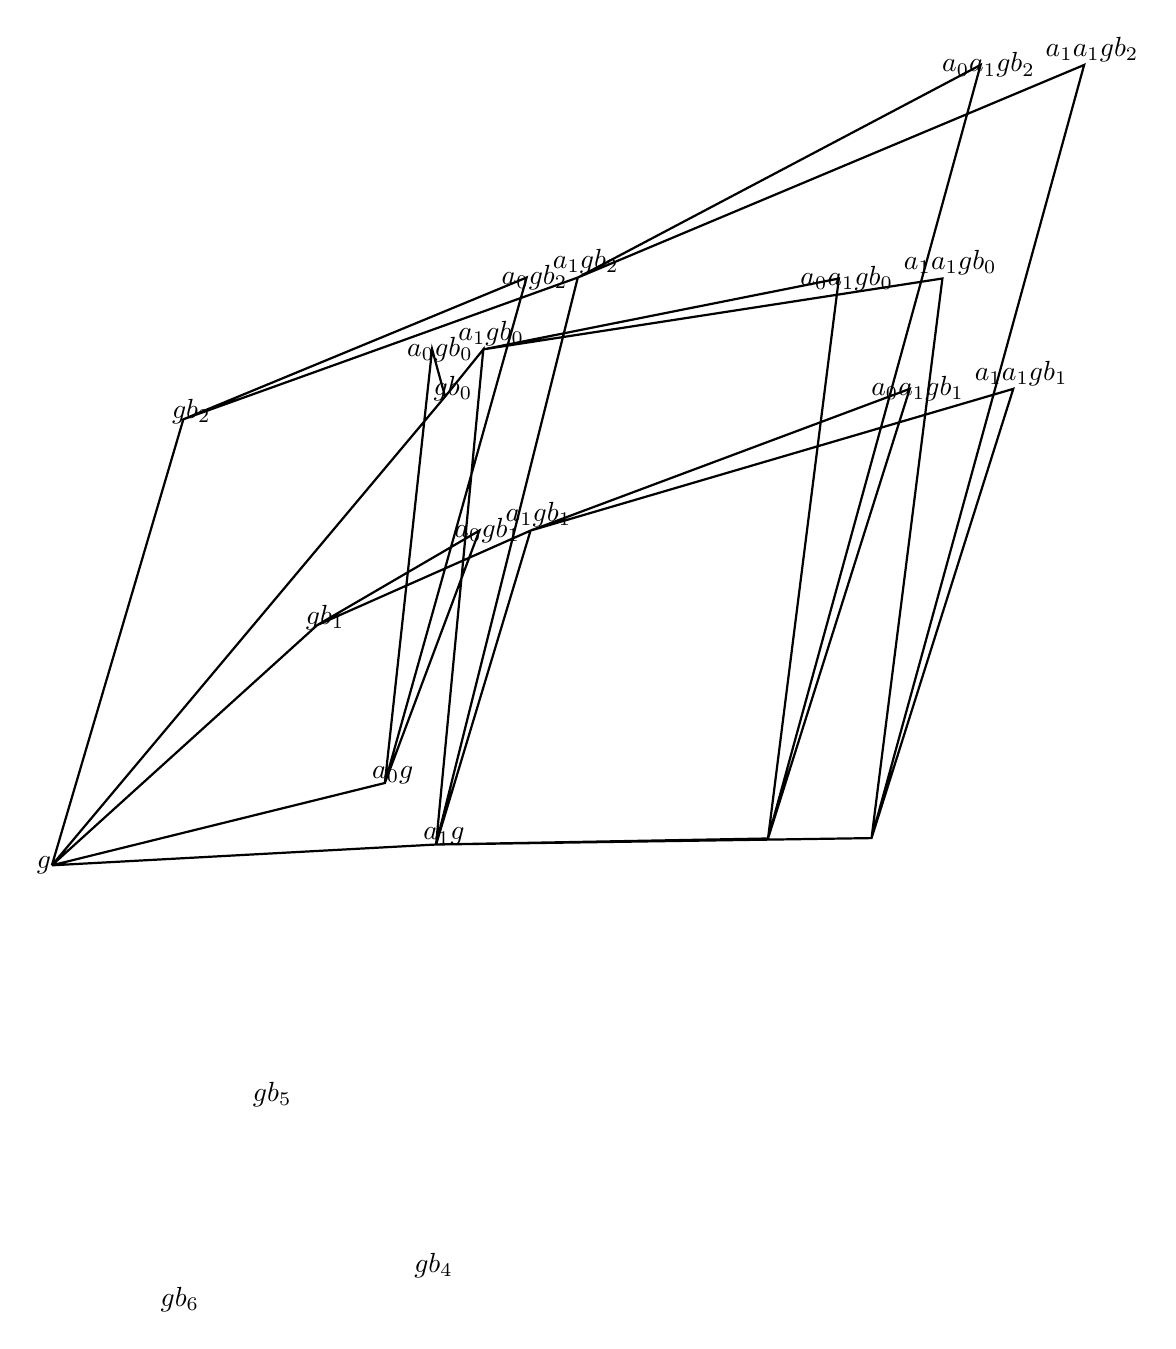
\begin{tikzpicture}
            \draw[thick](0,0)(0, 0) -- (4.993840581099619,5.952589633307452) -- (4.829073425795683,6.552589633307452) -- (4.229073425795684,1.0454686068434966) -- (0, 0)
(0, 0) -- (3.3706749841182475,3.051045119318713) -- (5.429073425795684,4.251045119318713) -- (4.229073425795684,1.0454686068434966) -- (0, 0)
(0, 0) -- (1.6700966131615953,5.664828105865107) -- (6.0290734257956835,7.464828105865107) -- (4.229073425795684,1.0454686068434966) -- (0, 0)
(0, 0) -- (4.993840581099619,5.952589633307452) -- (5.479211417777748,6.552589633307452) -- (4.879211417777748,0.2641838506026711) -- (0, 0)
(0, 0) -- (3.3706749841182475,3.051045119318713) -- (6.079211417777748,4.251045119318713) -- (4.879211417777748,0.2641838506026711) -- (0, 0)
(0, 0) -- (1.6700966131615953,5.664828105865107) -- (6.679211417777748,7.464828105865107) -- (4.879211417777748,0.2641838506026711) -- (0, 0)
(4.879211417777748, 0.2641838506026711) -- (5.479211417777748,6.552589633307452) -- (9.994981488229826,7.452589633307452) -- (9.094981488229825,0.34082138103510845) -- (4.879211417777748, 0.2641838506026711)
(4.879211417777748, 0.2641838506026711) -- (6.079211417777748,4.251045119318713) -- (10.894981488229826,6.0510451193187125) -- (9.094981488229825,0.34082138103510845) -- (4.879211417777748, 0.2641838506026711)
(4.879211417777748, 0.2641838506026711) -- (6.679211417777748,7.464828105865107) -- (11.794981488229826,10.164828105865107) -- (9.094981488229825,0.34082138103510845) -- (4.879211417777748, 0.2641838506026711)
(4.879211417777748, 0.2641838506026711) -- (5.479211417777748,6.552589633307452) -- (11.309719492364632,7.452589633307452) -- (10.409719492364632,0.345765132703422) -- (4.879211417777748, 0.2641838506026711)
(4.879211417777748, 0.2641838506026711) -- (6.079211417777748,4.251045119318713) -- (12.209719492364632,6.0510451193187125) -- (10.409719492364632,0.345765132703422) -- (4.879211417777748, 0.2641838506026711)
(4.879211417777748, 0.2641838506026711) -- (6.679211417777748,7.464828105865107) -- (13.109719492364633,10.164828105865107) -- (10.409719492364632,0.345765132703422) -- (4.879211417777748, 0.2641838506026711)
;
\node at (4.929073425795683,6.552589633307452) {$ a_{ 0  } gb_{ 0 } $};
\node at (5.5290734257956835,4.251045119318713) {$ a_{ 0  } gb_{ 1 } $};
\node at (6.129073425795683,7.464828105865107) {$ a_{ 0  } gb_{ 2 } $};
\node at (5.579211417777747,6.752589633307452) {$ a_{ 1  } gb_{ 0 } $};
\node at (6.179211417777748,4.451045119318713) {$ a_{ 1  } gb_{ 1 } $};
\node at (6.779211417777748,7.664828105865107) {$ a_{ 1  } gb_{ 2 } $};
\node at (10.094981488229825,7.452589633307452) {$ a_{ 0  } a_{ 1 }gb_{ 0 } $};
\node at (10.994981488229826,6.0510451193187125) {$ a_{ 0  } a_{ 1 }gb_{ 1 } $};
\node at (11.894981488229826,10.164828105865107) {$ a_{ 0  } a_{ 1 }gb_{ 2 } $};
\node at (11.409719492364632,7.652589633307453) {$ a_{ 1  } a_{ 1 }gb_{ 0 } $};
\node at (12.309719492364632,6.251045119318713) {$ a_{ 1  } a_{ 1 }gb_{ 1 } $};
\node at (13.209719492364632,10.364828105865106) {$ a_{ 1  } a_{ 1 }gb_{ 2 } $};
\node at (-0.1,0) {$ g $};
\node at (4.329073425795683,1.1454686068434967) {$ a_{ 0 }g $};
\node at (4.979211417777748,0.3641838506026711) {$ a_{ 1 }g $};
\node at (5.093840581099618,6.052589633307452) {$ gb_{ 0 } $};
\node at (3.4706749841182476,3.151045119318713) {$ gb_{ 1 } $};
\node at (1.7700966131615954,5.7648281058651065) {$ gb_{ 2 } $};
\node at (4.846847774934497,-5.087246295216067) {$ gb_{ 4 } $};
\node at (2.7979473340264533,-2.908459568425351) {$ gb_{ 5 } $};
\node at (1.6255391913540378,-5.510239172746165) {$ gb_{ 6 } $};

            \end{tikzpicture}
            \end{center}
            \caption{Square of the complex, with edges $(g,ag), (agb, gb) \in E_A,
            (g,gb), (agb, ag) \in E_B.$ \label{fig:square}
            }
            \end{figure}
 \begin{figure}[H]
            %\label{fig:square}
            \begin{center}
            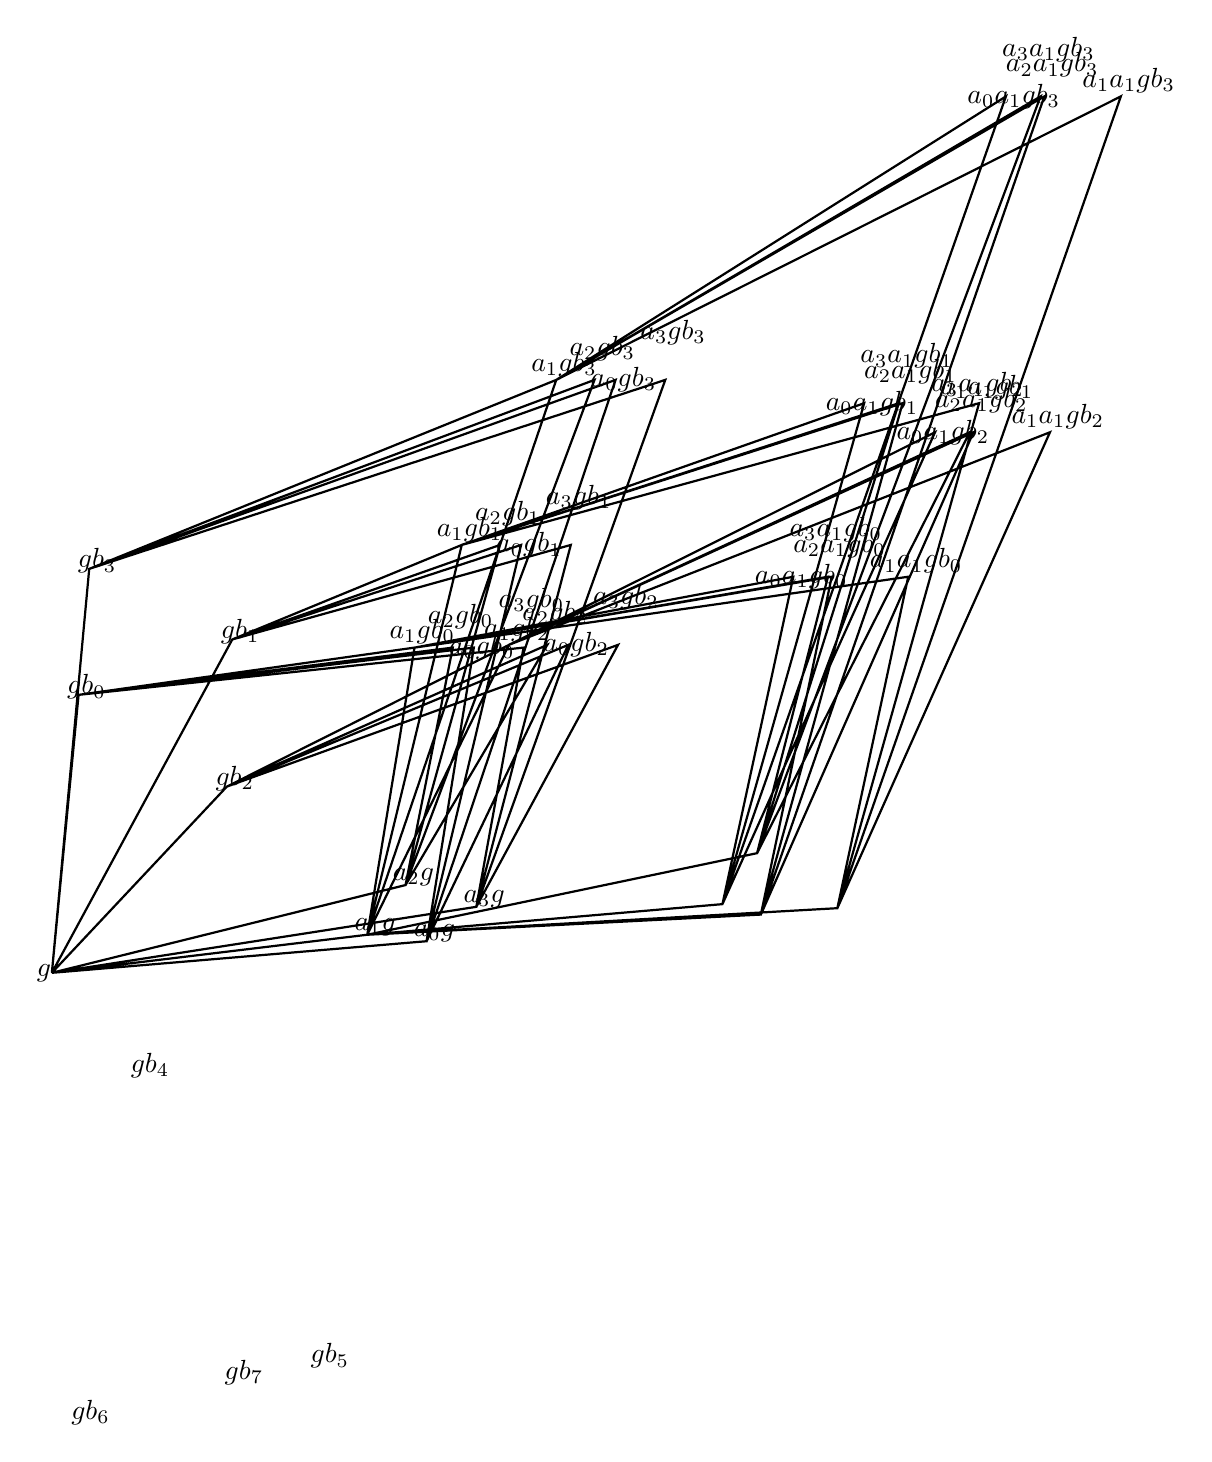
\begin{tikzpicture}
            \draw[thick](0,0)(0, 0) -- (0.3390511960785092,3.5300496501167746) -- (5.3588625046549225,4.130049650116774) -- (4.758862504654923,0.4013223858655578) -- (0, 0)
(0, 0) -- (2.2917381011818723,4.233948766487676) -- (5.958862504654923,5.433948766487676) -- (4.758862504654923,0.4013223858655578) -- (0, 0)
(0, 0) -- (2.2226541137369766,2.3649810686700627) -- (6.558862504654923,4.164981068670063) -- (4.758862504654923,0.4013223858655578) -- (0, 0)
(0, 0) -- (0.4743458432395731,5.1299675895446155) -- (7.158862504654923,7.529967589544615) -- (4.758862504654923,0.4013223858655578) -- (0, 0)
(0, 0) -- (0.3390511960785092,3.5300496501167746) -- (4.605476704022036,4.130049650116774) -- (4.005476704022036,0.48349157989767716) -- (0, 0)
(0, 0) -- (2.2917381011818723,4.233948766487676) -- (5.205476704022036,5.433948766487676) -- (4.005476704022036,0.48349157989767716) -- (0, 0)
(0, 0) -- (2.2226541137369766,2.3649810686700627) -- (5.805476704022036,4.164981068670063) -- (4.005476704022036,0.48349157989767716) -- (0, 0)
(0, 0) -- (0.4743458432395731,5.1299675895446155) -- (6.4054767040220355,7.529967589544615) -- (4.005476704022036,0.48349157989767716) -- (0, 0)
(0, 0) -- (0.3390511960785092,3.5300496501167746) -- (5.091354498418359,4.130049650116774) -- (4.491354498418359,1.1143087961869507) -- (0, 0)
(0, 0) -- (2.2917381011818723,4.233948766487676) -- (5.6913544984183595,5.433948766487676) -- (4.491354498418359,1.1143087961869507) -- (0, 0)
(0, 0) -- (2.2226541137369766,2.3649810686700627) -- (6.291354498418359,4.164981068670063) -- (4.491354498418359,1.1143087961869507) -- (0, 0)
(0, 0) -- (0.4743458432395731,5.1299675895446155) -- (6.891354498418359,7.529967589544615) -- (4.491354498418359,1.1143087961869507) -- (0, 0)
(0, 0) -- (0.3390511960785092,3.5300496501167746) -- (5.990210958081228,4.130049650116774) -- (5.390210958081228,0.8380359754576592) -- (0, 0)
(0, 0) -- (2.2917381011818723,4.233948766487676) -- (6.5902109580812285,5.433948766487676) -- (5.390210958081228,0.8380359754576592) -- (0, 0)
(0, 0) -- (2.2226541137369766,2.3649810686700627) -- (7.190210958081228,4.164981068670063) -- (5.390210958081228,0.8380359754576592) -- (0, 0)
(0, 0) -- (0.4743458432395731,5.1299675895446155) -- (7.790210958081229,7.529967589544615) -- (5.390210958081228,0.8380359754576592) -- (0, 0)
(4.005476704022036, 0.48349157989767716) -- (4.605476704022036,4.130049650116774) -- (9.416146678309145,5.030049650116775) -- (8.516146678309145,0.8721546208752922) -- (4.005476704022036, 0.48349157989767716)
(4.005476704022036, 0.48349157989767716) -- (5.205476704022036,5.433948766487676) -- (10.316146678309146,7.233948766487676) -- (8.516146678309145,0.8721546208752922) -- (4.005476704022036, 0.48349157989767716)
(4.005476704022036, 0.48349157989767716) -- (5.805476704022036,4.164981068670063) -- (11.216146678309144,6.864981068670063) -- (8.516146678309145,0.8721546208752922) -- (4.005476704022036, 0.48349157989767716)
(4.005476704022036, 0.48349157989767716) -- (6.4054767040220355,7.529967589544615) -- (12.116146678309144,11.129967589544615) -- (8.516146678309145,0.8721546208752922) -- (4.005476704022036, 0.48349157989767716)
(4.005476704022036, 0.48349157989767716) -- (4.605476704022036,4.130049650116774) -- (10.87560947030455,5.030049650116775) -- (9.97560947030455,0.8208383317075433) -- (4.005476704022036, 0.48349157989767716)
(4.005476704022036, 0.48349157989767716) -- (5.205476704022036,5.433948766487676) -- (11.77560947030455,7.233948766487676) -- (9.97560947030455,0.8208383317075433) -- (4.005476704022036, 0.48349157989767716)
(4.005476704022036, 0.48349157989767716) -- (5.805476704022036,4.164981068670063) -- (12.67560947030455,6.864981068670063) -- (9.97560947030455,0.8208383317075433) -- (4.005476704022036, 0.48349157989767716)
(4.005476704022036, 0.48349157989767716) -- (6.4054767040220355,7.529967589544615) -- (13.57560947030455,11.129967589544615) -- (9.97560947030455,0.8208383317075433) -- (4.005476704022036, 0.48349157989767716)
(4.005476704022036, 0.48349157989767716) -- (4.605476704022036,4.130049650116774) -- (9.904146913985427,5.030049650116775) -- (9.004146913985426,0.7396721351160819) -- (4.005476704022036, 0.48349157989767716)
(4.005476704022036, 0.48349157989767716) -- (5.205476704022036,5.433948766487676) -- (10.804146913985427,7.233948766487676) -- (9.004146913985426,0.7396721351160819) -- (4.005476704022036, 0.48349157989767716)
(4.005476704022036, 0.48349157989767716) -- (5.805476704022036,4.164981068670063) -- (11.704146913985426,6.864981068670063) -- (9.004146913985426,0.7396721351160819) -- (4.005476704022036, 0.48349157989767716)
(4.005476704022036, 0.48349157989767716) -- (6.4054767040220355,7.529967589544615) -- (12.604146913985426,11.129967589544615) -- (9.004146913985426,0.7396721351160819) -- (4.005476704022036, 0.48349157989767716)
(4.005476704022036, 0.48349157989767716) -- (4.605476704022036,4.130049650116774) -- (9.856141353446287,5.030049650116775) -- (8.956141353446286,1.5195334135177194) -- (4.005476704022036, 0.48349157989767716)
(4.005476704022036, 0.48349157989767716) -- (5.205476704022036,5.433948766487676) -- (10.756141353446287,7.233948766487676) -- (8.956141353446286,1.5195334135177194) -- (4.005476704022036, 0.48349157989767716)
(4.005476704022036, 0.48349157989767716) -- (5.805476704022036,4.164981068670063) -- (11.656141353446287,6.864981068670063) -- (8.956141353446286,1.5195334135177194) -- (4.005476704022036, 0.48349157989767716)
(4.005476704022036, 0.48349157989767716) -- (6.4054767040220355,7.529967589544615) -- (12.556141353446286,11.129967589544615) -- (8.956141353446286,1.5195334135177194) -- (4.005476704022036, 0.48349157989767716)
;
\node at (5.458862504654922,4.130049650116774) {$ a_{ 0  } gb_{ 0 } $};
\node at (6.058862504654923,5.433948766487676) {$ a_{ 0  } gb_{ 1 } $};
\node at (6.658862504654922,4.164981068670063) {$ a_{ 0  } gb_{ 2 } $};
\node at (7.258862504654923,7.529967589544615) {$ a_{ 0  } gb_{ 3 } $};
\node at (4.705476704022035,4.3300496501167745) {$ a_{ 1  } gb_{ 0 } $};
\node at (5.305476704022036,5.633948766487676) {$ a_{ 1  } gb_{ 1 } $};
\node at (5.9054767040220355,4.364981068670063) {$ a_{ 1  } gb_{ 2 } $};
\node at (6.505476704022035,7.729967589544615) {$ a_{ 1  } gb_{ 3 } $};
\node at (5.191354498418359,4.530049650116775) {$ a_{ 2  } gb_{ 0 } $};
\node at (5.791354498418359,5.833948766487676) {$ a_{ 2  } gb_{ 1 } $};
\node at (6.391354498418359,4.564981068670063) {$ a_{ 2  } gb_{ 2 } $};
\node at (6.991354498418358,7.929967589544615) {$ a_{ 2  } gb_{ 3 } $};
\node at (6.090210958081228,4.730049650116774) {$ a_{ 3  } gb_{ 0 } $};
\node at (6.690210958081228,6.033948766487676) {$ a_{ 3  } gb_{ 1 } $};
\node at (7.290210958081228,4.764981068670062) {$ a_{ 3  } gb_{ 2 } $};
\node at (7.890210958081228,8.129967589544615) {$ a_{ 3  } gb_{ 3 } $};
\node at (9.516146678309145,5.030049650116775) {$ a_{ 0  } a_{ 1 }gb_{ 0 } $};
\node at (10.416146678309145,7.233948766487676) {$ a_{ 0  } a_{ 1 }gb_{ 1 } $};
\node at (11.316146678309144,6.864981068670063) {$ a_{ 0  } a_{ 1 }gb_{ 2 } $};
\node at (12.216146678309144,11.129967589544615) {$ a_{ 0  } a_{ 1 }gb_{ 3 } $};
\node at (10.97560947030455,5.230049650116775) {$ a_{ 1  } a_{ 1 }gb_{ 0 } $};
\node at (11.87560947030455,7.433948766487676) {$ a_{ 1  } a_{ 1 }gb_{ 1 } $};
\node at (12.77560947030455,7.064981068670063) {$ a_{ 1  } a_{ 1 }gb_{ 2 } $};
\node at (13.675609470304549,11.329967589544614) {$ a_{ 1  } a_{ 1 }gb_{ 3 } $};
\node at (10.004146913985426,5.430049650116775) {$ a_{ 2  } a_{ 1 }gb_{ 0 } $};
\node at (10.904146913985427,7.633948766487676) {$ a_{ 2  } a_{ 1 }gb_{ 1 } $};
\node at (11.804146913985425,7.264981068670063) {$ a_{ 2  } a_{ 1 }gb_{ 2 } $};
\node at (12.704146913985426,11.529967589544615) {$ a_{ 2  } a_{ 1 }gb_{ 3 } $};
\node at (9.956141353446286,5.630049650116774) {$ a_{ 3  } a_{ 1 }gb_{ 0 } $};
\node at (10.856141353446287,7.833948766487676) {$ a_{ 3  } a_{ 1 }gb_{ 1 } $};
\node at (11.756141353446287,7.464981068670063) {$ a_{ 3  } a_{ 1 }gb_{ 2 } $};
\node at (12.656141353446285,11.729967589544614) {$ a_{ 3  } a_{ 1 }gb_{ 3 } $};
\node at (-0.1,0) {$ g $};
\node at (4.8588625046549225,0.5013223858655578) {$ a_{ 0 }g $};
\node at (4.105476704022036,0.5834915798976772) {$ a_{ 1 }g $};
\node at (4.591354498418359,1.2143087961869508) {$ a_{ 2 }g $};
\node at (5.490210958081228,0.9380359754576592) {$ a_{ 3 }g $};
\node at (0.4390511960785092,3.6300496501167747) {$ gb_{ 0 } $};
\node at (2.3917381011818724,4.3339487664876755) {$ gb_{ 1 } $};
\node at (2.3226541137369767,2.464981068670063) {$ gb_{ 2 } $};
\node at (0.574345843239573,5.229967589544615) {$ gb_{ 3 } $};
\node at (1.2465228104812205,-1.1764213056062087) {$ gb_{ 4 } $};
\node at (3.5307540337493686,-4.867005301396215) {$ gb_{ 5 } $};
\node at (0.49072596285280756,-5.580416268724132) {$ gb_{ 6 } $};
\node at (2.43977796229994,-5.078544563426938) {$ gb_{ 7 } $};

            \end{tikzpicture}
            \end{center}
            \caption{Square of the complex, with edges $(g,ag), (agb, gb) \in E_A,
            (g,gb), (agb, ag) \in E_B.$ \label{fig:square}
            }
            \end{figure}
 
%\end{multicols*}
  % \printbibliography 
\end{document}

 